\chapter{\textit{e-Tourism}}
\label{chp:eTourism}

O turismo é um setor de grande importância e que está sofrendo modificações com a inserção do comércio eletrônico como ferramenta para a realização de negócios. No Brasil, os dados de 2016 são: 6,6 milhões de turistas estrangeiros; 90,3 milhões de turistas nacionais; US\$ 6 bilhões de receitas diretas com o turismo interno. Segundo a mesma fonte, em 2015 houve US\$ 1.194 bilhões de receita cambial no turismo mundial \citep{embratur2016}.

Com a facilidade de acesso a rede e a ascensão dos dispositivos móveis, é cada vez mais necessário o desenvolvimento de sistemas que utilizem os recursos de mobilidade e de acesso à informação turística a qualquer hora e lugar. Nessa sessão, apresenta-se os principais conceitos envolvidos no trabalho e descrever trabalhos relacionados a sistemas de recomendações voltadas ao turismo.

\section{Introdução}
\label{sec:introductionETourism}

O avanço das tecnologias móveis e da Internet no nosso dia-a-dia vieram como uma maneira de revolucionar o comércio de produtos e serviços, permitindo rapidez e facilidade na hora de fazer uma compra, reduzindo os custos e o tempo. Isso modificou, de uma maneira geral, os mercados, seja de livros, músicas e jogos até entretenimento, como viagens, esportes, entre outros.

O comércio eletrônico revolucionou o anúncio, a distribuição, a venda e a informação de produtos turísticos, fazendo com que surgissem diversos sites especializados em turismo, seja para divulgar informações sobre bares, restaurantes, pontos turísticos e atrações das cidades, seja para facilitar na compra e venda de viagens, reserva de passagens, pousadas, hotéis e no transporte coletivo \citep{115416147001}. Diante dos números apresentados anteriormente, a Internet é uma ferramenta importante, pois contribui para a escolha de roteiros turísticos, representando investimento de tempo e dinheiro. Logo, o acesso as informações precisas e confiáveis são fundamentais para orientar o turista na escolha adequada \citep{115416147001}.

O turismo é uma atividade fortemente conectada com preferências pessoais e interesses das pessoas \citep{4669760}. Pensando nisso, o \textit{e-Tourism} vem como a possibilidade de personalizar a filtragem de informações, sugerindo ao usuário locais que são do interesse do mesmo, de acordo com suas preferências e outras variáveis (tempo disponível, programa para família ou individual, entre outros). \textit{e-Tourism} ou turismo eletrônico é definido como a digitalização de todos os processos e cadeias de valor da indústria do turismo, viagens, hotelaria e restauração que permitem às organizações maximizar sua eficiência e sua eficácia \citep{Moura:2013:DUT:2526188.2526215}.

\section{Sistemas de Informação para \textit{e-Tourism} e Classificações}
\label{sec:eTourism_infosys_classification}

Atualmente, muitas pessoas que planejam uma viagem procuram primeiramente a Internet para saber mais informações do local que pretendem visitar e programar suas as atividades. A Internet e as demais tecnologias tem facilitado bastante a vida das pessoas antes de uma viagem. Porém o visitante tem pouco conhecimento da cidade que irá visitar, além de não conhecer algumas atrações e os pontos turísticos que a cidade tem. Além disso, o usuário perde tempo para selecionar as atividades de sua preferência que ele pode fazer na cidade e organizá-los de forma que aproveite melhor o tempo disponível na viagem.

\subsection{Sistemas de Informação}
\label{subsec:eTourism_infoSys}

Existem diversos sistemas que disponibilizam informações de acordo com a entrada de preferências do usuário, entre eles os mais utilizados:

\begin{itemize}
    \item TripAdvisor\footnote{https://www.tripadvisor.com/}: é um site de turismo que auxilia em viagens, cidades para visitação e atividades para cada usuário e que também contém uma rede social, sendo possível adicionar \textit{reviews}, comentar e pontuar, ajudando no processo de tomada de decisões que pertence ao domínio do turismo.
    \item Booking.com\footnote{https://www.booking.com/}: site \textit{e-commerce} de viagens no mundo. Permite que você possa encontrar e reservar de uma maneira mais rápida a pousada ou hotel para a próxima viagem. Como diferencial, é possível procurar por hotéis próximos a localização ou próximo ao local que o usuário desejar. Por exemplo, se o turista está indo para a cidade de São Paulo, pode-se localizar hotéis próximos ao centro da cidade, ou ao Parque de Ibirapuera, entre outros.
    \item Foursquare\footnote{https://foursquare.com/}: uma rede social que ajuda de encontrar novas maneiras de explorar a cidade de acordo com as preferências de cada usuário. É possível fazer o \textit{check-in} da localização atual, classificar e deixar \textit{reviews} de locais.
\end{itemize}

\subsection{Classificação}
\label{subsec:eTourism_classification}

Encontram-se diversas formas de classificar os sistemas de recomendação para \textit{e-Tourism} \citep{BORRAS20147370}: pelas interfaces e por funcionalidades. A seguir, é discutido de forma mais detalhada como é feita essa classificação.

\subsubsection{Interfaces}
\label{subsubsec:eTourism_classification_interfaces}

A maioria dos sistemas de recomendação para turismo oferecem uma interface Web e/ou interface para dispositivos móveis. A interface Web permite que o usuário tenha uma maior interação com o sistema, visualizando as informações em mapas interativos, imagens e/ou vídeos de alta qualidade.  Como exemplo, o \textit{e-Tourism} \citep{4669760} mostra em um mapa os locais para serem visitados em um dia, de acordo com a programação.
Já o mobile permite que o usuário possa acessar as informações de qualquer lugar e utilizar de ferramentas que os dispositivos oferecem para incrementar o sistema na recomendação de locais para visitação (por exemplo, utilizar o GPS para saber da localização do turista e mostrar informações de pontos próximos a ele). O projeto \textit{ReRex} serviço que recomenda POIs para usuários mobile. \citep{Baltrunas2012}. Já o \textit{MTRS} \citep{Gavalas2011} é um sistema mobile que permite aos turistas construir roteiros customizados e oferece informações turísticas.

\subsubsection{Funcionalidades}
\label{subsubsec:eTourism_classification_functionalities}

Cada sistema de recomendação de turismo oferece diversas utilidades para o turista. Os mais comuns são:

\begin{itemize}
    \item Sugestão de destino e/ou construção de pacotes de turismo. O sistema tem como foco a recomendação de destinos que respeitem as preferências do usuário. No \textit{MyTravelPal} \citep{article} o turista é capaz de interagir em um mapa, no qual o sistema recomenda áreas de interesse na região. O tamanho do círculo indica o grau de afinidade com o usuário (Figura \ref{fig:recommended_municipalities}). Com foco em uma determinada área, é possível visualizar todos os locais e o tamanho depende da afinidade do perfil do viajante (Figura \ref{fig:recommended_tourist_objects}).
    \item Lista de classificação de atrações sugeridas: a maioria dos sistemas de recomendação de turismo fazem sugestões de pontos turísticos para o usuário que já decidiu para qual cidade viajará ou se ele já foi em um determinado local. Nesse caso, a classificação e pontuação dos pontos turísticos são de extrema importância para o sistema que tem disponível uma grande quantidade de informações para ser processada de acordo com as particularidades do usuário. Mais uma vez, o \textit{e-Tourism} \citep{4669760} é um bom exemplo de sistema de recomendação que utiliza uma lista de atividades que usuário deseja realizar, aquelas que já realizou além de locais que o turista já foi anteriormente.
    \item Planejamento de rotas: como já diz, sistemas desse tipo ajudam a criar rotas com uma lista de lugares de acordo com as preferências do turista. Para exemplificar o protótipo de \cite{Moura:2013:DUT:2526188.2526215} tem como foco traçar um itinerário no roteiro Caminhos da Pedra, na cidade de Bento Gonçalves, em que as atrações melhor avaliadas e relacionadas com os contextos do usuário possam ganhar mais visibilidade.
    \item Aspectos sociais. O sistema permite que os usuários compartilhem fotos, comentários, adicionarem uma pontuação ao local e interajam com outros turistas. Com isso, é possível recomendar locais analisando o \textit{score} e os comentários dos outros visitantes. O projeto \textit{e-Tourism} \citep{4669760} é um exemplo, que permite criar planos para visitação de locais de acordo com as preferências de um grupo de visitantes.
\end{itemize}

\begin{figure}
	\centering
	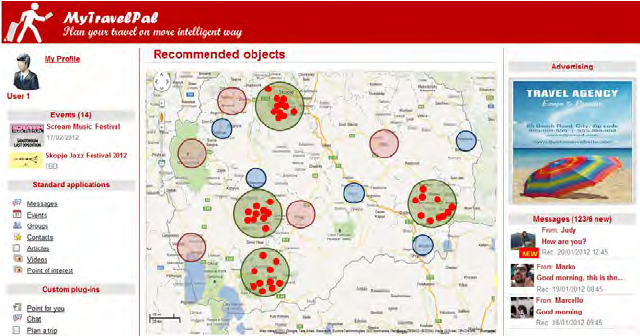
\includegraphics[scale=0.7]{images/Figure-no-1-Screenshots-of-the-recommended-municipalities.png}
	\caption{\textit{MyTravelPal}: mapa com recomendação de áreas de interesse \citep{article}.}
	\label{fig:recommended_municipalities}
\end{figure}

\begin{figure}
	\centering
	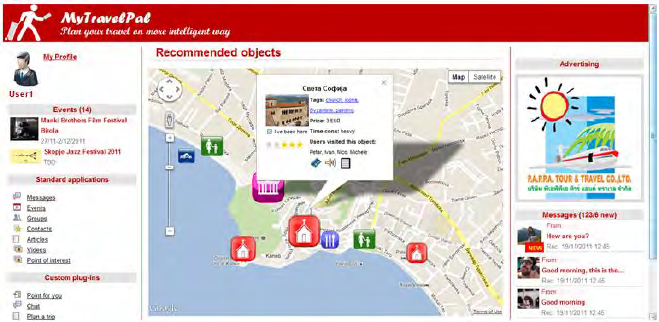
\includegraphics[scale=0.7]{images/Figure-no-2-Screenshots-of-recommended-tourist-objects.png}
	\caption{\textit{MyTravelPal}: mapa com recomendação de pontos turísticos e suas informações \citep{article}.}
	\label{fig:recommended_tourist_objects}
\end{figure}

\section{Sistemas de Recomendação para \textit{e-Tourism}}
\label{sec:eTourism_recsys}

Os sistemas de recomendação para turismo trazem pontos turísticos com base na individualidade de cada viajante. Cada sistema trabalha de uma maneira diferente na sugestão dos locais para o turista. Será apresentado três tipos de sistemas de recomendação para \textit{e-Tourism}: baseado em experiência de usuário, pontos de interesse e baseado em rotas.

\subsection{Sistemas de Recomendação Baseado em Experiência de Usuário}
\label{subsec:eTourism_recsys_userXP}

Os sistemas de recomendação baseados em experiência do usuário para \textit{e-Tourism} primeiramente verificam quais foram os pontos turísticos que o usuário já visitou antes, seja na cidade que ele deseja visitar, seja no histórico geral do turista, ou seja, pré-classificar alguns itens \citep{BORRAS20147370}. Com isso, é possível definir um gosto comum e, com essas informações, o sistema constrói um perfil inicial. 

Primeiramente, o sistema sugere locais que são parecidos com o que ele já visitou e o usuário marca as atrações do seu agrado e desmarca aquelas que ele não aprovou. Após a visita do turista nas atrações, este pode opinar deixando um \textit{feedback} ou uma pontuação sobre o local. O processamento do \textit{feedback} do usuário é muito importante pois é através das informações obtidas das suas avaliações que o sistema de recomendação melhora o perfil do turista e pode oferecer pontos que mais se adaptam ao seu gosto \citep{4669760}.

Um exemplo disso é o \textit{e-Tourism}, um sistema que constrói um itinerário de acordo algumas características e restrições do usuário para a visita, como o período, o tempo destinado para a visitação, se estará sozinho ou com a família, além do local de origem, idade e gênero \citep{4669760}.

\subsection{Sistemas de Recomendação de Pontos de Interesse}
\label{subsec:eTourism_recSys_poi}

O rápido crescimento e desenvolvimento das cidades proporcionou um número muito grande de pontos de interesse (conhecido na língua inglesa como \ac{poi}), como por exemplo restaurantes, hotéis, lojas, entre outros. Diante de uma larga quantidade de POIs, o usuário tem problemas de fazer uma decisão satisfatória de "onde ir" de acordo com seus interesses pessoais. Sistemas de Recomendação de Pontos de Interesse tem como objetivo resolver um destes problemas ajudando os usuários a filtrar os POIs mais importantes e reduzir o tempo gasto para fazer uma decisão \citep{AAAI159560}.

O desenvolvimento de redes sociais baseada em localização (\ac{lbsn}) permite que sistemas de recomendação de POIs em LBSNs possam estudar os comportamentos do usuário mobile para recomendação de POIs de acordo com aspectos de espaço, de tempo, sociais e de conteúdo. Através dos \textit{check-ins} dos usuários nas redes sociais de geolocalização utilizando \textit{smartphones}, é possível visualizar quem, quando, onde e o que foi marcado como ponto de interesse \citep{AAAI159560}.

As informações contidas nos LBSNs pode estar relacionados a ação de \textit{check-in} do usuário, promovendo uma única oportunidade para sistemas de recomendação baseadas em POIs. Como exemplo, verificando a descrição de um POI que contém "churrascaria", conclui-se que este restaurante tem como prato principal carnes vermelhas e usuários que fazem \textit{check-in} neste POI talvez tenham interesse em churrasco. Este é um exemplo de propriedade de POI. Isso mostra que recomendações de POIs para um usuário baseado nas suas ações através de \textit{check-ins} leva em consideração as informações disponíveis, como exemplo, interesses do usuário e propriedades de POIs.

O \textit{framework} desenvolvido em \cite{AAAI159560} para recomendação de pontos de interesse leva em conta também indicações de sentimento do usuário no POI. No exemplo anterior, o POI da churrascaria pode conter comentários de diversos usuários sobre o local, elogiando ou deixando uma reclamação, seja da comida ou do serviço prestado pelo estabelecimento. Nessa pesquisa, foi utilizado os \textit{check-ins} da rede social \textit{Foursquare}\footnote{http://sendible.com/insights/what-is-foursquare-location-based-social-networking}, uma das mais populares LBSN.

Em muitos sistemas de recomendação baseado em filtragem colaborativa utilizando POIs, são considerados somente os pontos de interesse que o usuário ou seus amigos já visitaram, não funcionando corretamente quando inclui pontos que anda não foi visitados. Para contornar esse problema, \cite{Ying:2012:UPR:2346496.2346507}, propôs o \textit{Urban POI-Mine (UPOI-Mine)}, que tem como objetivo criar um sistema de recomendações baseado em filtragem colaborativa utilizando POIs. Foram utilizados três aspectos complementares para extrair características dos POIs dos usuários: fator social, preferencia individual e popularidade do POI.

O aspecto fator social corresponde a oferecer POIs para o usuário de acordo com todos os \textit{check-ins} entre os seus amigos que contém preferências similares, considerando análises estatísticas. As preferências individuais capturam relações entre usuários e POIs, explorando as atividades de \textit{check-ins} do usuário para pontos de interesse com as mesmas propriedades. Porém, esses dois aspectos podem não funcionar corretamente para novos usuários pois informações de \textit{check-ins} são bem escassas. A popularidade dos POIs é incluída para maximizar a estimativa de semelhança da relação entre usuário e POI. Por exemplo, pessoas podem ir todos os dias a uma churrascaria, mas raramente vão a um restaurante oriental. Pensando assim, estima-se a equivalência por probabilidade condicional, que é a probabilidade de os usuários irem a um determinado ponto, de acordo com a categoria. Isto é chamado de popularidade relativa do POI.

Um outro exemplo é o de \cite{Ye:2011:EGI:2009916.2009962}, que além de utilizar a influência social dos amigos do usuário, utiliza-se também a influencia geográfica. \cite{Ye:2011:EGI:2009916.2009962} verificou que os usuários tendem a visitar POIs próximos, seja do trabalho ou de casa, ou de um ponto que esteja próximo da sua atual localização, mesmo que seja longe de casa. Essa análise impactou mais na recomendação de pontos de interesse em LBSNs comparado com a influência social.

\subsection{Sistemas de Recomendação Baseado em Rotas}
\label{subsec:eTourism_recSys_routes}

Existem diversas ferramentas de navegação e transporte que oferecem serviços de rotas baseados na localização do usuário. Como exemplo o \textit{Google Maps}\footnote{https://maps.google.com} extrai a localização através do GPS do celular ou utilizando tecnologias alternativas. Essa é uma das principais características de um sistema de recomendação baseado em rotas: construir uma rota capaz de atender as necessidades do usuário com diferentes focos \citep{GAVALAS2014319}.

Um dos focos é oferecer a menor rota de POIs recomendados próximos da atual localização do usuário. É possível utilizar informações de redes sociais (com \textit{tags} e pontuações colaborativas) para providenciar recomendações de rotas personalizadas \citep{GAVALAS2014319}. Outro ponto são passeios turísticos personalizados, como exemplo, lista ordenada de atrações ao longo de um ponto de origem e destino, de acordo com as preferências do usuário e outras variáveis: atual posição do turista, tempo disponível, interesses de viagem, passeios a pé personalizados, entre outros \citep{GAVALAS2014319}.

Mais um foco são sistemas de recomendação baseado em rotas que englobam meios de transporte, considerando todos os serviços disponíveis na cidade, como metrô, ônibus, a pé, bicicleta, trem, etc. Para isso, o sistema pode criar rotas que utilizam diversos meios de transporte através de um conjunto de POIs ou primeiro gerar o passeio turístico e depois gerar a rota considerando as conduções disponíveis \citep{GAVALAS2014319}. Como exemplo, o UbibusRoute é um sistema móvel que considera informações contextuais dinâmicas do trânsito através de redes sociais, apresentando dados sobre as rotas de ônibus aos usuários \citep{lima2012ubibusroute}.

\begin{table}[h!]
    \centering
	\caption{Análise dos sistemas de recomendação \textit{e-Tourism}.}
	\label{tab:analise_tourism_recommender}
	\begin{tabular}{|r|p{11cm}|}
		\hline
		\multicolumn{1}{|c|}{\bfseries Característica} & \multicolumn{1}{|c|}{\bfseries Referências} \\ \hline
		
		Interface & \cite{4669760}, \cite{Baltrunas2012}, \cite{Gavalas2011}. \\ \hline
		Funcionalidades & \cite{article}, \cite{4669760}, \cite{Moura:2013:DUT:2526188.2526215}. \\ \hline
		Experiência de Usuário & \cite{4669760}.	\\ \hline
		Pontos de Interesse & \cite{AAAI159560}, \cite{Ying:2012:UPR:2346496.2346507}, \cite{Ye:2011:EGI:2009916.2009962}, \cite{Gavalas2011}, \cite{Baltrunas2012}. \\ \hline
		Rotas & \cite{lima2012ubibusroute}, \cite{Moura:2013:DUT:2526188.2526215}. \\ \hline

	\end{tabular}
\end{table}

\section{Sumário}
\label{sec:summaryETourism}

Neste capítulo introduziu-se o \textit{e-Tourism}, mostrando suas aplicações e características. A Tabela \ref{tab:analise_tourism_recommender} mostra um resumo dos sistemas de recomendação de turismo citadas neste capítulo e suas devidas características, classificadas de acordo com as categorias apresentadas anteriormente. Os próximos capítulos estão organizados da seguinte maneira: O Capítulo \ref{chp:eTourismRecSys} apresenta a proposta de aplicação de sistemas de recomendação baseado em filtragem colaborativa em sugestões de rotas de pontos turísticos e discute como foi feita a implementação. O Capítulo \ref{chp:evaluation} apresenta a avaliação da ferramenta e no Capítulo \ref{chp:conclusion} conclusões e considerações finais.